\chapter{Feature Engineering}
\label{chap:fea}

\todoA{FEATURE SELECTION FOR
KNOWLEDGE DISCOVERY AND
DATA MINING
Huan Liu
Hiroshi Motoda}


As we said we cannot straightforwardly use the raw data form training our classifier.
Instead, we will represent each instance with a set of features, each feature expressing a certain property about the instance.
An example of a feature can be number of words in the review,\
a feature expressing whether word {\it food} is present in the review
or a feature extracting some metadata, like how many stars the user gave.

Features are divided by their values into three categories~---~nominal, ordinal and continuous. Nominal features are discrete and their values do~not convey any relationship. When a~feature is ordinal, it means it is discrete and also convey ordering of the values. Continuous feature is then any real-valued variable.

In this text we will deal with nominal and ordinal only. The simplest way to treat ordinal features is to omit the order. This of course loses information conveyed in this ordering, but will allow us easier feature manipulation.

\section{Extraction}

When we come up with feature we want to use, we often have to do some preprocessing and then computing the value of a feature for each particular instance.
This process is called {\bf feature extraction}.
We will use features like number of words and therefore we need to split the reviews into words first.
This is called {\bf tokenization}, because we are splitting the text into tokens (words in this context).
We will use Tweet tokenizer from the library nltk.
The reason we use it is that it does not only split words by spaces,
but also punctuation and considers punctuation signs to be tokens as well.
This allows the features to carry some potentially useful information.
An example is indication that a word as at the end of a sentence if it is followed by a full stop.

Subsequently, it is often needed to convert words into lower case and {\it lemmatise} them.
Both these techniques are used to group words that express the same meaning together.
The case of lower case is clear.
{\bf Lemmatisation} means replacing a word with its lemma, which is a kind of {\it base form} of the word.
The reason of doing this is to group inflected words together.
An example in English is {\it car} and {\it cars}.
Both words clearly express the same property and we may want to group them together.
Of course, the exact meaning is different, but often for purposes of classification known that there is a car
suffices. It is not necessary to known whether one or more.
Because English is not highly inflectional language, we will omit this process and use only lower case conversion.


\todoA{ref to nltk.}


\section{Selection}

Machine learning is used in contexts where the true natural and inner logic of~data is~not known.
Therefore it is difficult to intuitively select only useful features and we often extract as many features as we can hoping some of them will be useful.
Having too many features can lead to undesirable effects and only those features that are in some respect useful are passed to the training phase.

Having fewer features which are informative enough leads to three direct benefits.
Trained model is far less complex and as~such easier to~interpret.
The~model also generalises better, because the~risk of overfitting is lower.
Overfitting happens when the~model recognises irregularities in training data and classifies individual already seen instances, whereas it should approximate the~original model to~be able to~classify unseen instances.
Lastly, fewer features result in shorter training time.

Three methods of feature selection are generally recognised.


\subsection{Filters}

The main objective of filters is to filter out not so much informative features. It evaluates {\it informativness} of each feature individually and ...

Filters are popular, because their time complexity is linear in the~number of~features. However, the feature selection may~not be optimal, because neither the~used classificator nor feature correlation is taken into account. When there are highly correlated features, it is unnecessary to choose all of them, because the information conveyed in some may be inferred from others. However, any filter will choose all of them, because filters consider features independently of each other.

Filters work with individual features independently of any supervised classification algorithm. Each feature is used or omitted based on the filter condition. There are number of filters differing in the filter condition.

\subsubsection{Mutual Information}

As \citet{Hoq14} defines it, {\bf mutual information}~$I(X, Y)$~is the amount of uncertainty in X due to the knowledge of Y. It is defined as:

$$sum p(x,y) log(p(x,my)/op(x)/p(y)$$

It can be also expressed as

$$I(X, Y) = H(X) - H(X|Y),$$

where~$H(x)$~is entropy of random variable~$X$~and~$H(X|Y)$~the conditional entropy.
This way~$H(X)$~expresses the of uncertainty of~$X$~and~$H(X|Y)$~what~$Y$~does not say about~$X$.
This supports the intuitive idea that information gain expresses how much information one variable carries about the other one.

The basic approach is to compute mutual information of each feature and the class label.
Only feature exceeding some given threshold are then used for training.
\citet{Hoq14} proposes improved algorithm.
Instead of choosing all feature in one step, they choose one feature at a time and repeat this process until again a given threshold is exceeded.
Two values are calculated for each not selected feature.
First, feature-class as in the basic approach.
Second, the average of mutual information between the feature all already used features.
Then they choose such a feature that has the highest feature-class and also lowest average of feature-feature.
This prevents including highly correlated features into training set.
We have not used this approach due to the lack of time and used the basic approach.



\subsubsection{Chi-square~---~$\chi^2$}

Chi-square test of independence can be thought of
as a measure of the lack of independence between two variables.
As in mutual information,
we will compute a special value for each pair feature-class
and based on some threshold we will choose the most informative features.
Let us demonstrate this with an example.
We have instances of our reviews and we want to test how well
a feature \textit{contains the phrase ``credit card''} describes
labels \textit{useful} and \textit{not-useful}.
To asses this, we want to compute~$\chi^2$ of the variables~$X$~and~$Y$.
First, representing the feature \textit{contain ``credit card''}.
Second, the true label.

Table~\ref{tab:chi_ex} summaries this.
The inner cells express how many instances there are with the given variable values.
The bottom most row and right most column express marginal probability distribution 
calculated by the number of samples.
If the variables very truly independent,
we would expect the cells to be 15 and 35 in the first and second row respectively.
We will introduce a cost function to reflect this
and~$\chi^2$~of the two variables will then be sum of the cost function over all cells.


\todoA{aligning and crop excess vertical lines}
\begin{table}[h!]
 \center
 \begin{tabular}{|l|l|c|c|c}
 \cline{3-4}
        &       & \multicolumn{2}{c|}{label} & \\
        \cline{3-4}
        &       & yes        & no            & $P_Y$ \\
        \cline{1-4}
 credit & yes   & 25         & 5             & 0.30 \\
        \cline{2-4}
 card   & no    & 45         & 25            & 0.70 \\
        \cline{1-4}
        & $P_X$ & 0.50       & 0.50          & 1
 
 \end{tabular}
 \caption{$\chi^2$~Example}
 \label{tab:chi_ex}
\end{table}

The exact definition can be found in \citet{Hugh13}.
Let us have two random variables~$X$~and~$Y$.
Let us define~$O_{x,y}$ and~$E_{x,y}$~as the number of observed,
resp. expected instances for~$X=x$~and~$Y=y$.
The value of~$O_{x,y}$~is simply the number of instances.
The value of~$E_{x,y}$ is computed from marginal probabilities.
Namely:

\begin{equation}
E_{x,y} = P_X\left(X=x\right) P_Y\left(Y=y\right) \times n,
\end{equation}

where~$P_X$~and~$P_Y$~are the marginal probabilities of the variables~$X$~and~$Y$
and~$n$~number of all instances.

We define $\chi^2$~of two random variables~$X$~and~$Y$~as:

$$\sum_{x \in X, y \in Y}{\chi^2_{y,x}},$$

where~${\chi^2_{y,x}}$ is $\left(O_{x,y} - E_{x,y} \right)^ 2 / E_{x,y}$.

This corresponds to our intuition.
If the variables are correlated,
the observed values will differ from expected and~$\chi^2$ will by non-zero.
The farther observed value from the expected is, the higher penalization with square.
Also, it is normalized by dividing it in E.

The value of $\chi$ in our example in the table~\ref{tab:chi_ex}
~is:

\begin{equation}
\chi^2 = 
\frac{\left(25-15\right)^2}{15} +
\frac{\left(5-15\right)^2}{15} +
\frac{\left(45-35\right)^2}{35} +
\frac{\left(25-35\right)^2}{35}
\end{equation}

\begin{equation}
\chi^2 \approx 11
\end{equation}


\todoB{advantages/dis... a bit of discussion}

\subsection{Wrappers}

Unlike filters, wrappers work with subsets of features and use a classifier to directly asses informativness.
Every subset is classified by a classificator used as a black box and then evaluated by some common evaluation metrics.
The optimal subset is than chosen. Thanks to this, wrappers are universal and robust.

Furthermore, wrappers can perform a lot better than filters on certain datasets. Such a~case is documented by \citet{GuyEli03} in~\ref{fig:guyeli03-figure3}. The bottom left graph shows the original data and the~top left shows projection onto only one axis. It is clear that one variable cannot be sufficient for separating the clusters. However, if we project the data onto a combination of the two axis, the clusters can be at least partially separated as can be seen in the right part of the figure.
 
 \todoA{citation and vector}

\begin{figure}[ht]\centering
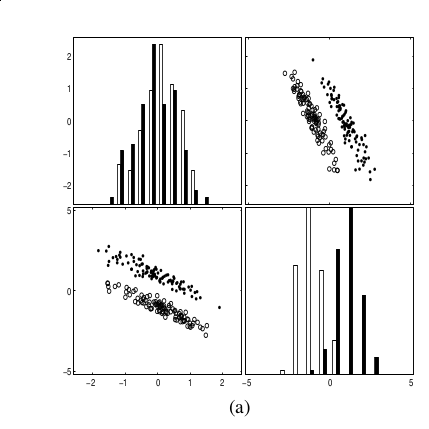
\includegraphics[width=100mm]{../img/guyeli_figure3.png}
\caption{Example of correlated features from the article}
\label{fig:guyeli03-figure3}
\end{figure}

Unfortunately, wrappers tend to be computationally expensive, because every subset must by classified separately. In fact, it has been shown it is NP-hard to find optimal solution. To achieve computational feasibility various approximation methods has been developed. These methods allow us to classify only a fraction of subsets at the cost of losing the guarantee of the optimal solution. We will describe two variants of greedy search.

\todoB{On the approximability of minimizing nonzero variables
or unsatisfied relations in linear systems --- citation of the NP-hard, otherwise delete} 

\subsubsection{Greedy Search --- Forward Selection}

{\it Forward selection} starts with an empty set and in every step adds a feature which brings the highest gain in the evaluation metrics. The feature is selected by adding all of them to the current  subset and evaluating it. The step is repeated until the increase in performance is less than a certain threshold. 

\subsubsection{Greedy Search --- Backward Elimination}

{\it Backward elimination} starts with the set of all features. In one step every feature is removed from the subset and this new subset is than evaluated. The feature which decreased the evaluation the least will be removed. This step is repeated until the evaluation drops by more than a given threshold. This approach may be infeasible for really big data sets, but includes all useful features of which some may be omitted by forward selection.




\subsection{Embedded Methods}

Embedded methods are part of a classification algorithm itself. An example can be a decision tree, which takes features that lower the entropy the most first. More on this in particular algorithms.

\todoA{The last sentence should be removed if there are no such algos in this doc.}

\section{Singular Value Decomposition (SVD/PCA)}

 - not feature selection, nor extraction
 - as an intermediate process between training and extracting/selecting

\section{Commonly Used Features}

In this section we will use some commonly used features and briefly discuss their pros and cons.

\subsection{Bag-Of-Words}
\label{subsec:bow}

Since the information a sentence carries is not contained only in the words, but also in their positions in the sentence, an ideal algorithm would take into account both the words and their positions.
However, working with sentences as a whole is somewhat difficult. Hence, the order of words is often omitted and only the number of word occurrences matters.
This approach is called {\bf Bag-Of-Words} (BOW). Bag-Of-Words for an instance is simply a mapping of every word onto the number of occurrences in the given text.

\subsubsection{TF-IDF}

In a general document there are many words that are not directly useful.
{\it TF--IDF} is a way to evaluate which words are the most important for individual documents.  
\citet{SalBuc88} describe the motivation for introducing this.
The goal is to select such words that it will be define the document well enough, yet leaves enough room for describing all relevant documents.
We will introduce two metrics to convey these two requirements and then use a combination of those two to gain the best results.

First, we will simply use only words occurring enough times in a document. This is referred to as {\it term-frequency}.
We will introduce {\it inverse-document frequency} (IDF) to skip words such as {\it an}, {\it the} which appear in virtually every sentence and carry very little information.
IDF is indirectly proportional to the number of documents which contain a given word.
Thanks to this, words like articles will be given very little weight.

There are many implementations of this general idea. We will explore the implementation described in \citet{Ramos03}. Given a set of documents~$D$, word~$w$ and an individual document~$d$,
we can calculate TF-IDF as

\[
	w_d = TF \times IDF = f_{w, d} \times \log \left( \frac{\abs{D}}{f_{w,D}}  \right),
\]

where $TF = f_{w, d}$ is the number of times~$w$~occured~$d$ and IDF corresponds to $\log \left( \frac{\abs{D}}{f_{w,D}}  \right)$ for $\abs{D}$ being the total number of documents and $f_{w, D}$ the number of documents containing~$w$.

Let us explore how the value changes with different variable values. For such words that $\abs{D} \sim f_{w, D}$ will the value of logarithm very low. This will decrease the importance of the word. This is desired behaviour because such words occur in virtually every document and, as argued above, are not very useful. On the other hand, words having $f_{w,d}$ large and $f_{w,D}$ will be given much higher importance, which is again desired, because these words occur relatively often in the given document and not so often in the document set overall.

\todoA{Is this really the way we're going to use it? We have very short texts}

\todoA{- TD*IDF - with given threshholds - how to find it?}

\todoB{try TD*IDF not with a~given threshold, but rather find te optimal threshold for cuts}

\subsection{N-grams}

When using BOW, we can potentially loose useful information conveyed in the word order.
Unfortunately, it is often computationally infeasible to retain the complete order.
To find a balance between these two issues, {\bf N-grams} try to convey the order only partially.
{\bf N-gram} is simply a sequence of items, in our case words. The~$N$~refers to the length of the sequence.
The longer a sequence is to more order is preserved at higher computational cost.
Bigrams and trigrams (pairs and triples) are most commonly used.

\todoB{- choose words with highest information gain; as in McCallum Event models}

\subsection{Word Embeddings}
\label{subsec:wordembed}

Word Embeddings is another way to convert words into features.
\citet{LeGo14} describe {\bf word embedding} as a mapping of every word to a vector in~$R^d$.
This is also sometimes referred to as distributed word representation.
This mapping is obtained by using a big corpus of data by optimizing some cost function.

\citet{Mik13} showed that if parameters are set carefully, word embeddings conveys both semantic and sytanctic information.
First, similar words are mapped to similar vectors. So we can measure a sort of synonymity.
Not only that, but it also conveys relations between words.
An example they show is singular vs plural. Let~$x_{w}$ be the vector of the word~$w$.
Than then showed that $x_{apple}-x_{apples} \sim x_{car}-x_{cars}$.
Even more complicated relations like $x_{king} - x_{man} + x_{woman} \sim x_{queen}$ where shown.
They use this property to solve word analogies in form {\it a is to b as c is to \_\_\_}.


\subsection{Geneea entities}

\bf entities extracted from geneea \rm

 \todoB{- filter them based on the~geneea value of importance}

 \todoA{- occurrences - pick only the~most frequent}

\subsection{\todoB{Cosine sim}}


\subsection{hand crafted features}

\subsubsection{\todoA{Spell check}}

\subsubsection{\todoA{Review length}}

\subsection{non-textual features --- metadata}

\todoB{Stars as non-linguistic feature}

